%%% Sekce - Nákupní košík
%%%%% Wording: ✅
%%%%% Styling: ✅
%%%%% References: ✅
%%% --------------------------------------------------------------
\section{Nákupní košík}
\label{sec:identifikace-nakupni-kosik}
Velmi důležitou součástí fungování celého systému je efektivní správa a vizualizace nákupního košíku.
Ta například zákazníkovi poskytuje přehledný souhrn položek, které si objednává, a umožňuje mu je případně upravit či odebrat, jak je znázorněno na obrázku~\ref{fig:ticketportal-cart}.
Jedním z nejzásadnějších aspektů nákupního košíku jsou jaká data jsou v něm uchovány a jakým způsobem jsou zpracována.

Tato sekce se zabývá popisem hlavních funkčností a požadavků na nákupní košík, které jsou nezbytné pro jeho efektivní fungování v rámci webového řešení s využitím rezervace sedadel.

\begin{figure}[H]
    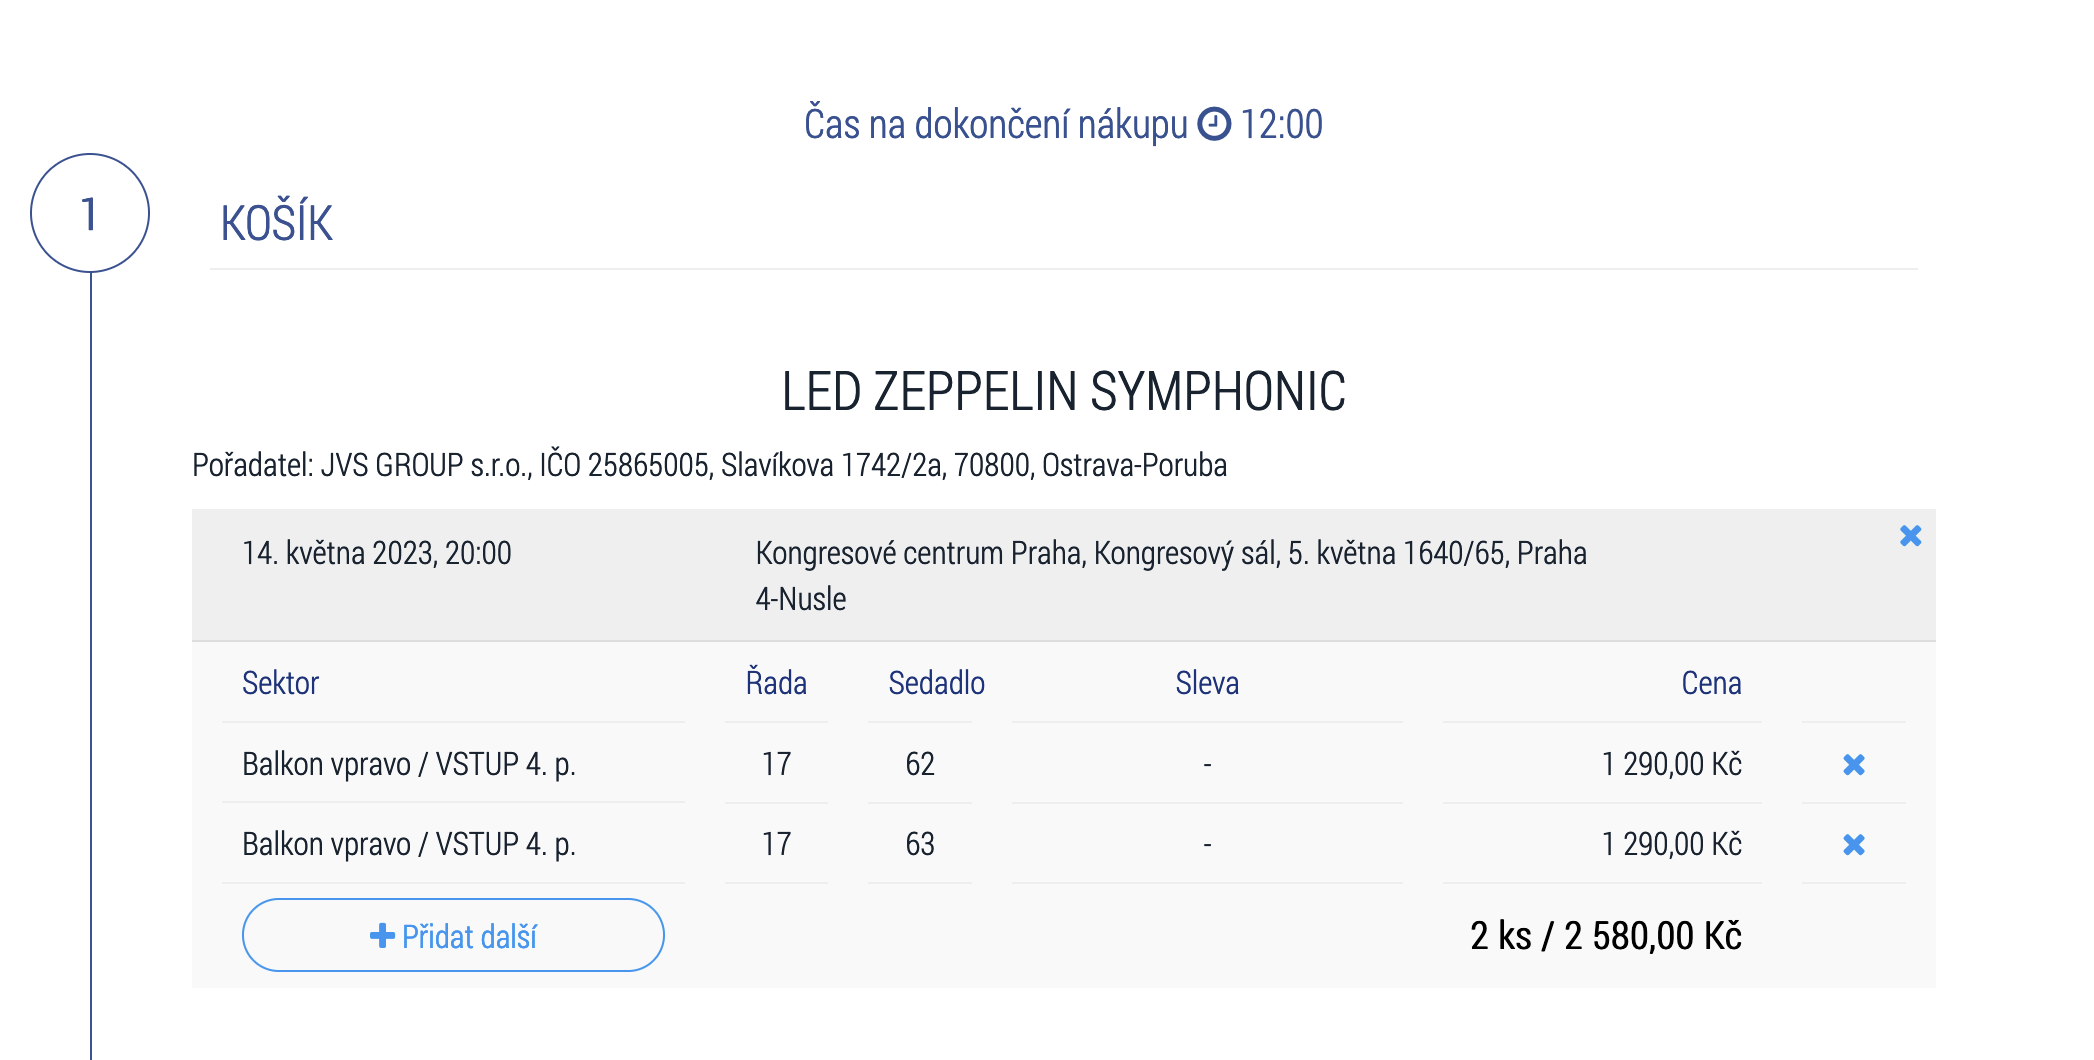
\includegraphics[width=\linewidth]{\FIGDIR/ticketportal-cart}
    \centering
    \caption{Obsah nákupního košíku na portálu Ticketportal.cz\cite{t__www_ticketportal_cz}}
    \label{fig:ticketportal-cart}
\end{figure}

%%% Podsekce - Správa dat
%%%%% Wording: ✅
%%%%% Styling: ✅
%%%%% References: ✅
%%% --------------------------------------------------------------
\begin{subsection}{Správa dat}
    \label{subsec:identifikace-nakupni-kosik-sprava}
    Nákupní košík by z datové perspektivy měl být implementován jako objekt, který uchovává informace o všech vybraných sedačkách a vstupenkách.
    Datová struktura a uchovávaná data uvnitř daného objektu o stavu nákupního košíku by měla být jasně definovaná a dostupná ve formátu vyhovujícímu užití aplikace.
    Díky těmto datům by mělo být vždy možné zrekonstruovat stav nákupního košíku a to i v případě, že uživatel opustí stránku nebo zavře prohlížeč.

    Touto problematikou se bude primárně zabývat kapitola~\ref{sec:implementace-kosik}, ve které bude podrobně popsána datavá struktura a finální funkčnost nákupního košíku.
\end{subsection}

%%% Podsekce - Přehled obsahu košíku
%%%%% Wording: ✅
%%%%% Styling: ✅
%%%%% References: ✅
%%% --------------------------------------------------------------
\begin{subsection}{Přehled obsahu košíku}
    \label{subsec:identifikace-nakupni-kosik-prehled}
    Pro zákazníka nákupní košík slouží primárně k přehlednému zobrazení všech vybraných položek, které budou tvořit jeho objednávku.
    V případně této webové aplikace se primárně jedná o vstupenky a zarezervované sedačky.

    Zákazník by měl být schopen jednoduše zjistit, jaké položky si objednává a jaké mají parametry.
    Seznam všech těchto položek posléze tvoří celkový přehled nákupního košíku, který umožňuje zákazníkovi zkontrolovat jeho výběr a provést případné změny před dokončením objednávky.
    Ukázka přehledného obsahu nákupního košíku je znázorněna na obrázku~\ref{fig:ticketmaster-cart-overview}, kde je zobrazen seznam všech vybraných vstupenek včetně jejich parametrů.

    \begin{figure}[H]
        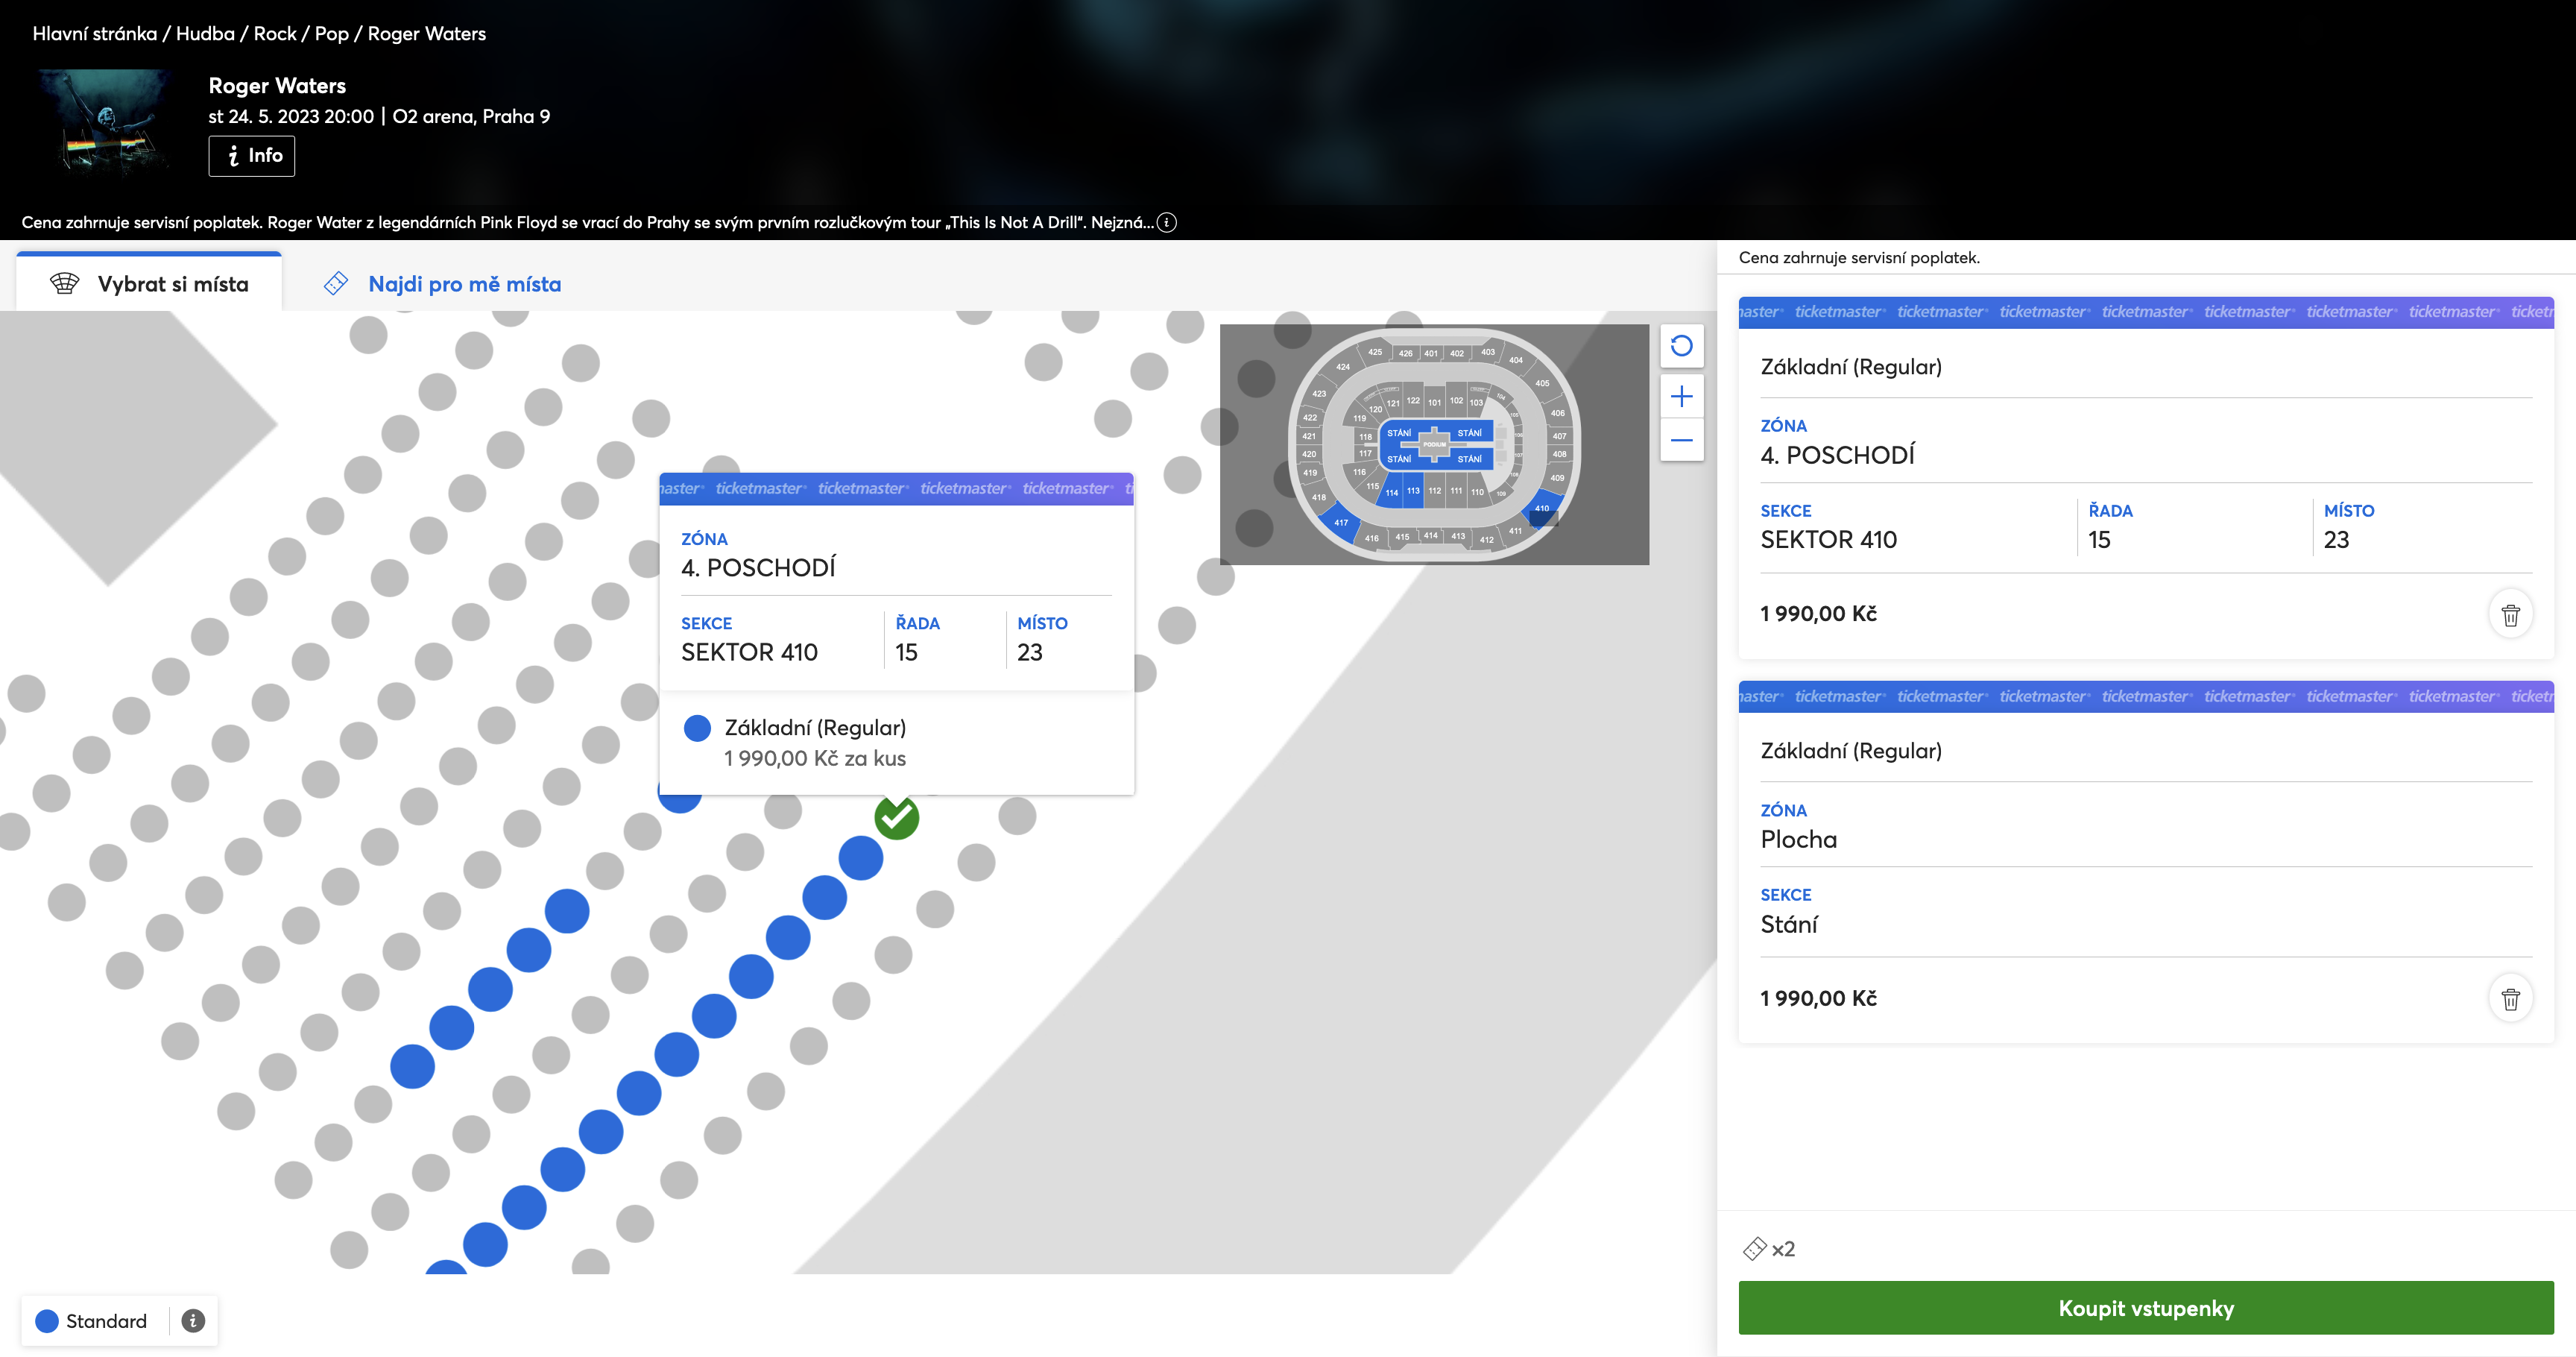
\includegraphics[width=\linewidth]{\FIGDIR/ticketmaster-cart-overview}
        \centering
        \caption{Nákupní košík na portálu Ticketmaster.com\cite{t__www_ticketmaster_com}}
        \label{fig:ticketmaster-cart-overview}
    \end{figure}

    Nákupní košík by zároveň měl zobrazit přehled cen jednotlivých položek a celkovou cenu objednávky včetně všech daní a dalších případních poplatků.
    Tato funkcionalita zákazníkovi zajišťuje naprostou transparentnost v nabízených službách a umožňuje mu předem zkontrolovat celkovou cenu objednávky.
    V dalším kroku objednávkového procesu v síti Ticketmaster.com je zákazníkovi zobrazen souhrn objednávky, který obsahuje všechny výše zmíněné informace.
    Tento souhrn je znázorněn na obrázku~\ref{fig:ticketmaster-cart-summary}.

    \begin{figure}[H]
        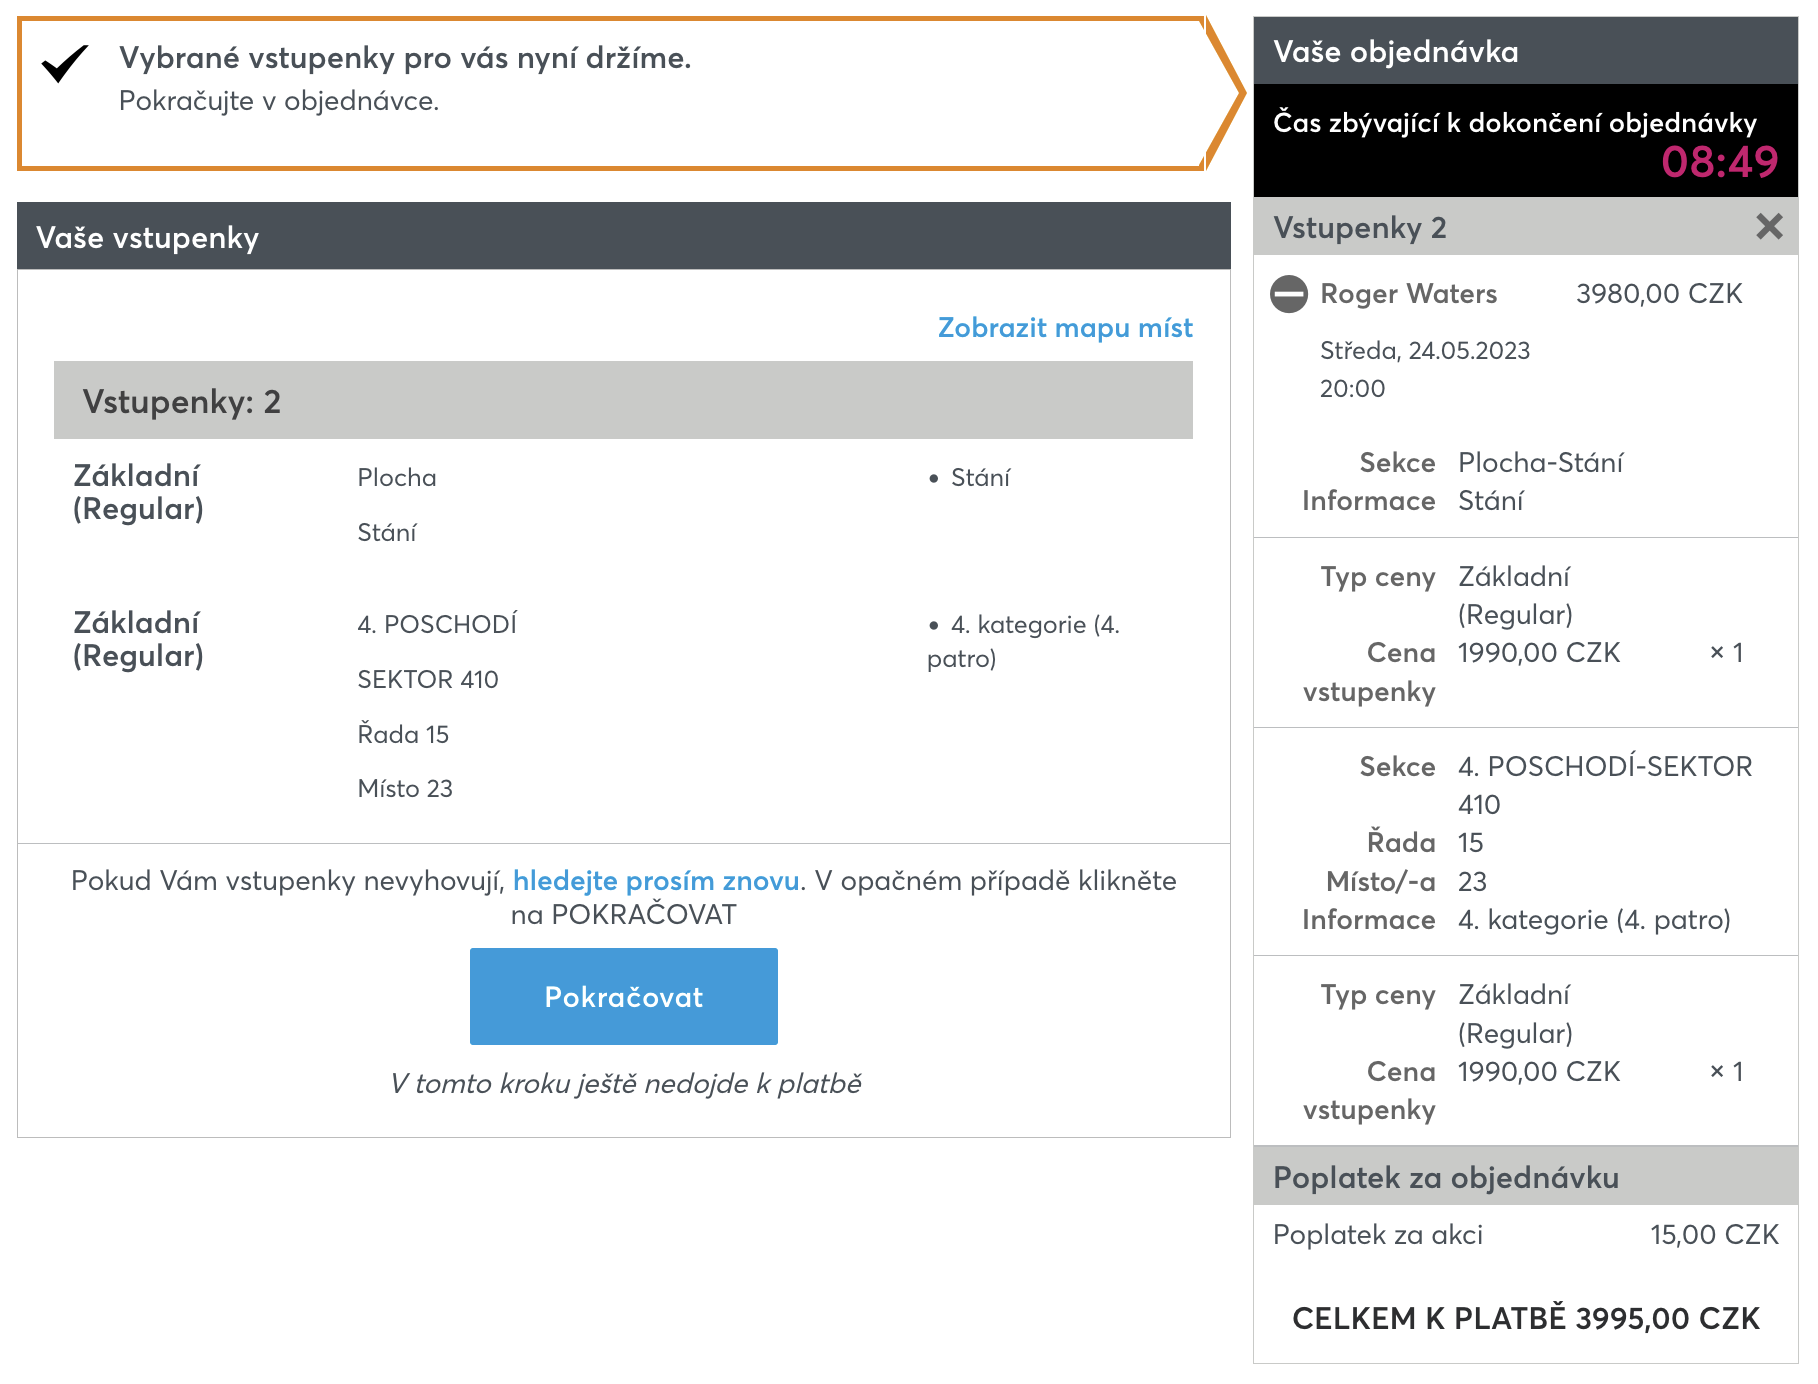
\includegraphics[width=\linewidth]{\FIGDIR/ticketmaster-cart-summary}
        \centering
        \caption{Souhrn objednávky na portálu Ticketmaster.com\cite{t__www_ticketmaster_com}}
        \label{fig:ticketmaster-cart-summary}
    \end{figure}
\end{subsection}

%%% Podsekce - Rezervace míst
%%%%% Wording: ✅
%%%%% Styling: ✅
%%%%% References: ✅
%%% --------------------------------------------------------------
\begin{subsection}{Rezervace míst}
    \label{subsec:identifikace-nakupni-kosik-rezervace}
    V rámci nákupního procesu si zákazník vybírá místa, které jsou dostupná a při jejich výběru se zákaznikovi přidají do nákupního košíku.
    Tato vybraná místa zákazníkem by se měla rezervovat, aby se předešlo nepříjemným situacím při dokončení objednávky, kdy zákazník zjistí, že jeho vybrané místo je již obsazené.

    V případně aplikace, která se primárně zaměřuje na rezervací míst při prodeji vstupenek je tato funkcionalita naprosto esenciální.
    Zákazník by měl mít možnost vybrat si místa, která jsou v danou chvíli dostupná a při jejich výběru by se měla pomocí rezervačnícho mechanismu v rámci vytvářené objednávky zákazníkovi zarezervovat a garantovat mu v případně dokonení objednávky jejich dostupnost.

    Tento rezervační systém by měl dále implementovat funkčnost časového omezení rezervace, která zajistí uvolnění rezervovaných míst po uplynutí určitého časového limitu.
    Tato funkčnost je velmi důležitá pro zajištění dostupnosti míst pro všechny zákazníky a zabraňuje zarezervování sedadel, která by nebyla zakoupena například z důvodu opuštění nákupního procesu zákazníkem.

    V rámci tohoto rezervačního mechanismu by také mělo být zákazníkovi jasně zobrazeno, že má určitý časový limit, ve rámci kterého musí svou objednávku dokončit, jinak se jeho rezervace uvolní a bude si muset místa vybrat znovu.
    Názořným příkladem takového rezervačního systému může být služba NFCtron Tickets, která je znázorněna na obrázku~\ref{fig:nfctron-tickets-reservation}.

    \begin{figure}[H]
        \centering
        \begin{subfigure}{0.3\textwidth}
            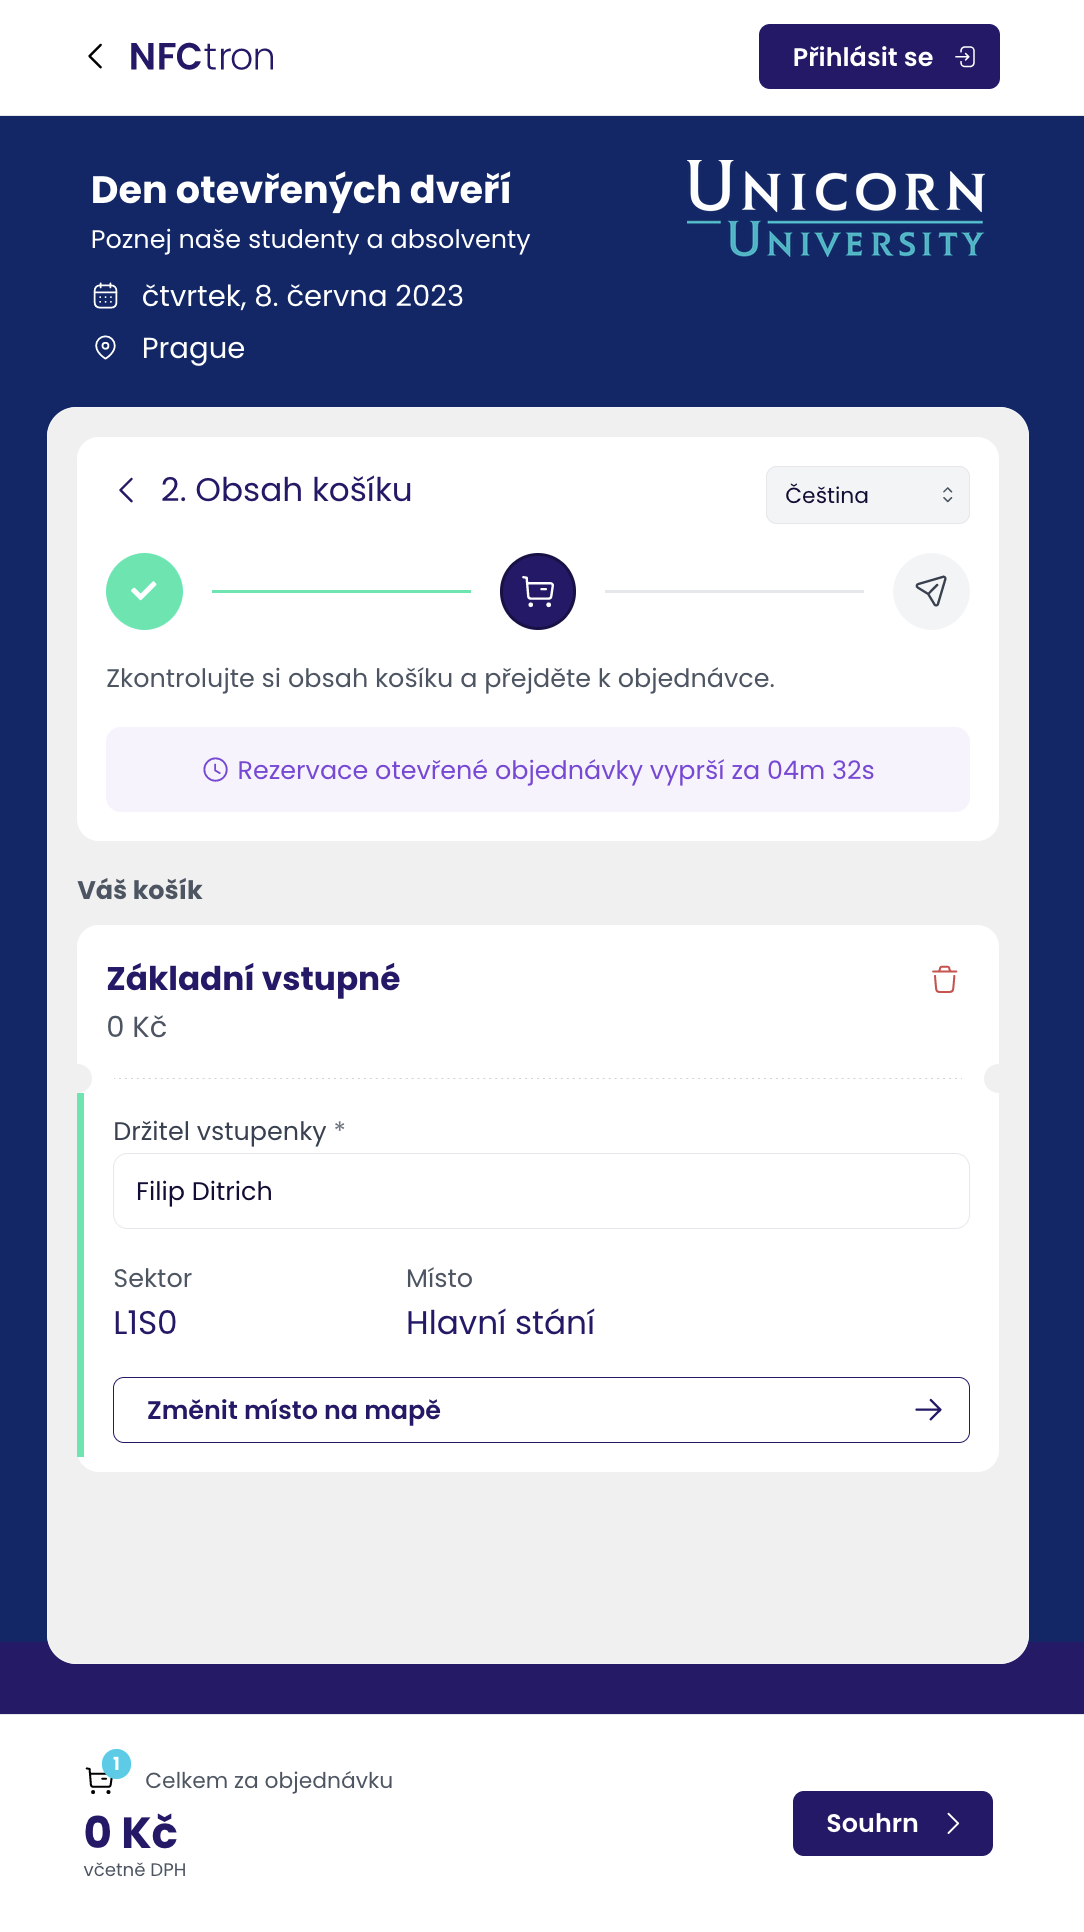
\includegraphics[width=\textwidth]{\FIGDIR/nfctron-tickets-reservation-pending}
            \caption{Běžící rezervace}
            \label{fig:nfctron-tickets-reservation-pending}
        \end{subfigure}
        \hfill
        \begin{subfigure}{0.3\textwidth}
            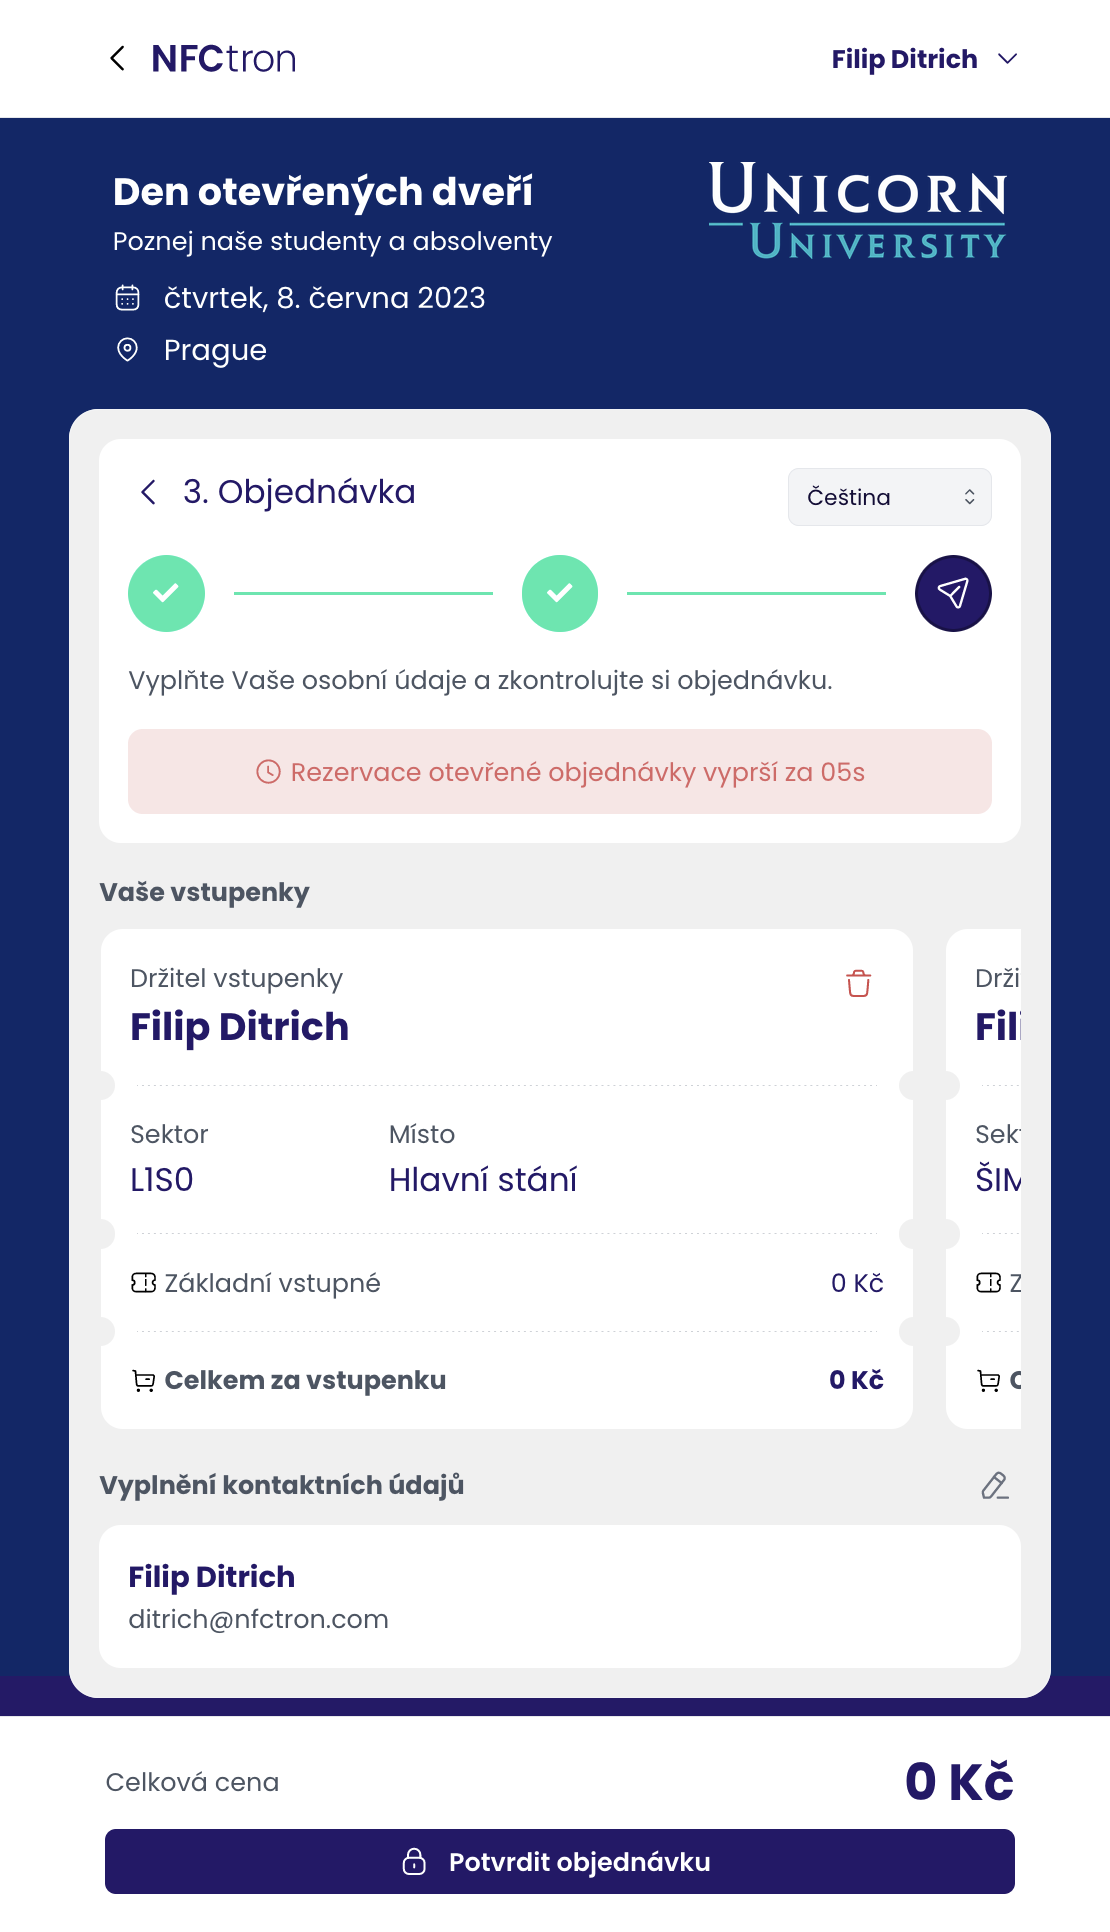
\includegraphics[width=\textwidth]{\FIGDIR/nfctron-tickets-reservation-expiring}
            \caption{Blížící se expirace}
            \label{fig:nfctron-tickets-reservation-expiring}
        \end{subfigure}
        \hfill
        \begin{subfigure}{0.3\textwidth}
            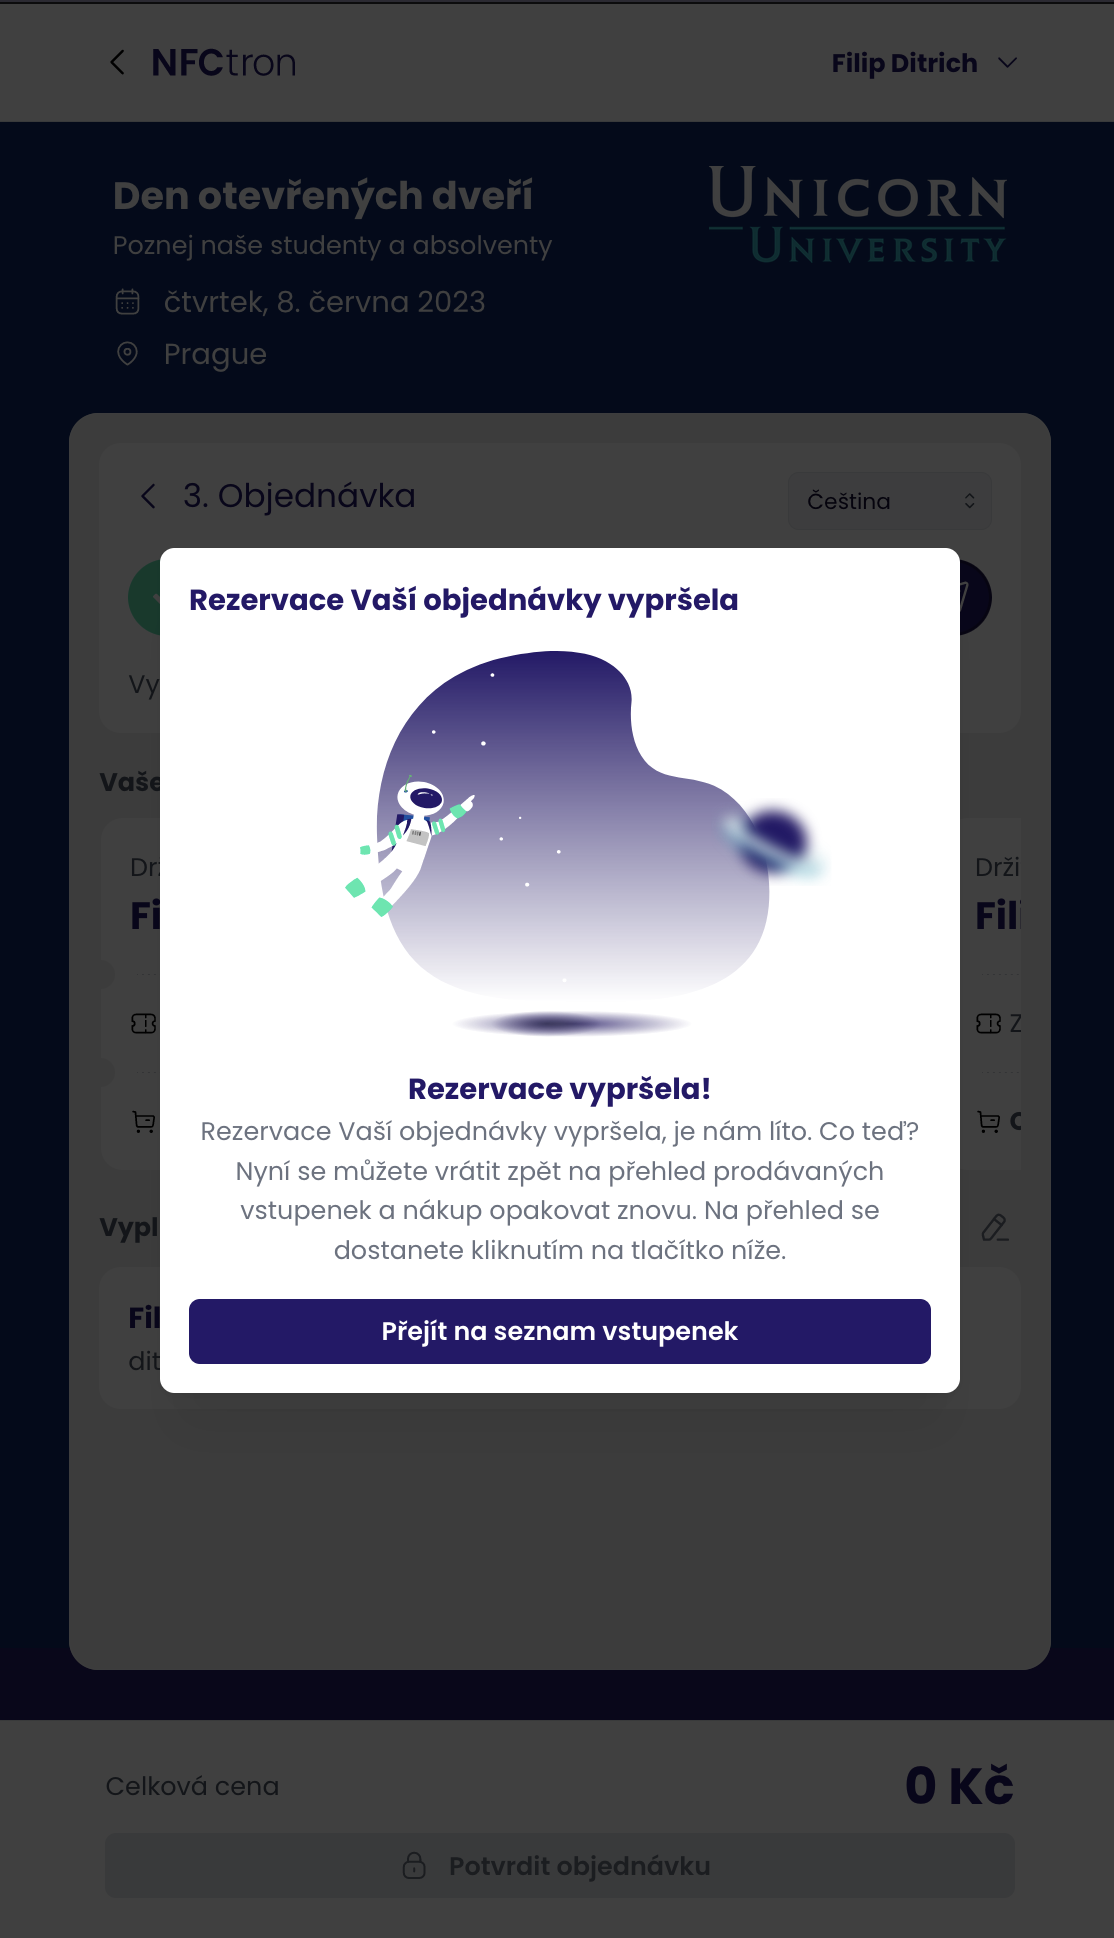
\includegraphics[width=\textwidth]{\FIGDIR/nfctron-tickets-reservation-expired}
            \caption{Expirovaná rezervace}
            \label{fig:nfctron-tickets-reservation-expired}
        \end{subfigure}

        \caption{Rezervační mechanismus služby NFCtron Tickets na zkušební akci\cite{nt_nfctron_simonfest}}
        \label{fig:nfctron-tickets-reservation}
    \end{figure}
\end{subsection}
